% !TEX root = main.tex

\section{存储器的层次结构}
\subsection{概述}
存储器按照存储方式可分为以下几种:
\begin{enumerate}
	\item 随机访问存储器(RAM)\\
	存储器任意单元可随时访问且访问所需时间相同
	\begin{itemize}
		\item 静态(SRAM):cache\\
		\textbf{触发器}(寄存器也是);只要加电源,信息就能一直保持;集成度低,引脚多,速度快\\
		一般由以下几个部分组成:
		\begin{itemize}
			\item 存储阵列(存储体)
			\item 译码器电路
			\item 控制电路:$\overline{CE}$(Chip Enable), $\overline{WE}$(Write Enable), $\overline{OE}$(Output Enable)(后两个通常可合并)
			\item 数据缓冲电路
		\end{itemize}
		\item 动态(DRAM):主存\\
		\textbf{电容};每隔一段时间必须刷新;现在一般用DDR3 SDRAM(Double Data-Rate Synchronous)\\
		\begin{itemize}
			\item 分散式/异步刷新:在最大刷新间隔前将所有行刷新一遍
			\item 集中刷新
			\item 透明式刷新:每访存一次刷新一次
		\end{itemize}
	\end{itemize}
	\item 只读存储器(ROM):都采用随机存取方式进行访问;BIOS(Basic Input Output System)\\
	正常工作时只读,能随机读出,不能随机写入
	\begin{itemize}
		\item MROM:掩模式,只读
		\item PROM:一次性编程
		\item EPROM/EEPROM:多次改写,后者为电可擦除可编程存储器
	\end{itemize}
	\item 相联存储器(Content Addressed Memory, CAM):\textbf{快表(TLB)}\\
	按\textbf{内容}检索到存储位置进行读写
	\item 直接存取存储器(DAS):磁盘\\
	可以直接定位到要读写的数据块,存取时间的长短与数据所在位置有关
	\item 顺序存储器(SAS):磁带、电荷耦合器件CCD、VCD\\
	数据按顺序从存储载体的始端读出或写入,存取时间的长短与数据所在位置有关
\end{enumerate}
基本术语:
\begin{itemize}
	\item 记忆单元/存储位元/位元(Cell):具有两种稳态的能够表示二进制数0和1的物理器件
	\item 存储单元/编址单位(Addressing Unit):存储器中具有\textbf{相同地址}的那些位构成一个存储单元,又称为一个编址单位
	\item 存储体/存储矩阵/存储阵列(Bank):所有存储单元构成一个存储阵列
\end{itemize}
\begin{center}
存储位元 $\to$ 存储单元 $\to$ 存储矩阵 $\to$ 存储芯片(译码、驱动、读/写电路) $\to$ 存储模块(内存条) $\to$ 存储器
\end{center}
按照信息的可保存性分为:
\begin{itemize}
	\item 断电后数据是否丢失
	\begin{itemize}
		\item 挥发性(volatile)/易失存储器:SRAM、DRAM
		\item 非挥发性/非易失存储器(NVM):ROM、磁盘、闪存
	\end{itemize}
	\item 读出后是否保存数据
	\begin{itemize}
		\item 破坏性存储器(读出原信息被破坏,需重写):DRAM
		\item 非破坏性存储器:SRAM
	\end{itemize}
\end{itemize}
地址译码两种方式
\begin{enumerate}
	\item 线选法(一位地址译码)\\
	SRAM,只在单方向译码,同时读出一条字线上的所有位,$k$位地址对应$2^k$地址驱动线
	\item 位片式(二维双译码)\\
	$k$位地址对应$2^\frac{k}{2}+2^\frac{k}{2}$条地址驱动线\\
	若行列地址线复用,则可表示$2^{2k}$个地址
\end{enumerate}
\begin{example}
某一SRAM芯片,容量为1024$\times$8位,除电源和接地端外,该芯片数据与地址引脚的最小数目为?
\end{example}
\begin{analysis}
$1024B=2^{10}B$,故需10条地址线,8位则8条数据线,外加1条片选信号和1条读写控制线,共20条
\end{analysis}
\begin{example}[2014全国统考]
某容量为256MB的存储器由若干4M$\times$8位的DRAM芯片构成,该DRAM芯片的地址引脚和数据引脚总数是?
\end{example}
\begin{analysis}
片选信号不需理,$4MB=2^{22}B$,故需22条地址线,又其为DRAM地址复用,故只需11条\\
加上8条数据线,共19条
\end{analysis}
\begin{figure}[H]
\centering
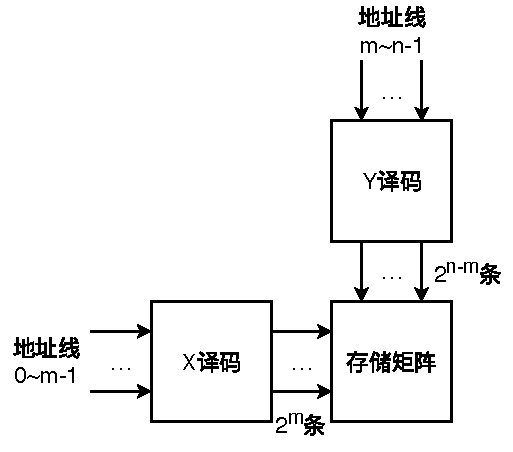
\includegraphics[width=0.4\linewidth]{fig/Memory-Double_Decode.pdf}
\end{figure}
存储器读写的时序:横线在中间为高阻,斜线为任意值,空白为有效
\begin{itemize}
	\item SRAM:行列地址同时送\\
	地址有效$\to$片选有效$\to$数据有效$\to$片选无效$\to$地址无效
	\begin{figure}[H]
	\centering
	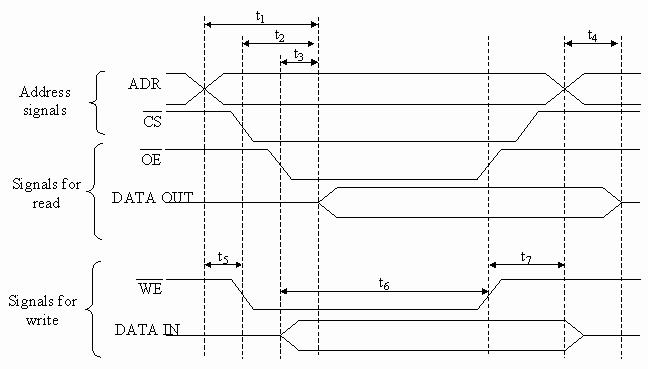
\includegraphics[width=0.4\linewidth]{fig/sram_cycle.png}
	\end{figure}
	\item DRAM:地址复用\\
	行地址有效$\to$行地址选通$\to$列地址、数据有效$\to$列地址选通$\to$数据输入$\to$全部无效
\end{itemize}
\begin{itemize}
	\item 读出时间$T_r$:从发出地址读命令到将数据读出来所需时间
	\item 存取周期$T_s$:连续两次读出两个主存单元所需的最小时间间隔(如DRAM要重写再生),$T_s<T_r$
\end{itemize}
多个请求同时读写存储器
\begin{itemize}
	\item 双端口存储器(时间并行):同时读写不同存储单元没有问题
	\item 多模块交叉存储器(空间并行):每个体都有自己的MAR、MDR和读写电路,可独立并行工作
	\begin{itemize}
		\item 连续编址(高位交叉):用主存地址码高位区分体号,低位表示模块内地址;存储地址连续的数据落在同一存储体内,易发生访存冲突(同时访问一个存储体),并行可能性小
		\item 交叉编址(低位交叉):以存储体个数(质数)为模交叉编址,把连续几个地址保存到不同存储器中;CPU同时送出m个地址,高位作为存储器地址,低位负责选择数据;由存储器分时使用数据总线进行信息传递(流水线)
	\end{itemize}
\end{itemize}
\begin{example}[2017全国统考]
某计算机主存按字节编址,由4个64M$\times$8位的DRAM芯片用交叉编址方式构成,并与宽度为32位的存储器总线相连,主存每次最多读写32位数据。若double型变量x的主存地址为804001AH,则读取x需要的存储周期数为?
\end{example}
\begin{analysis}
低位交叉编址,没有对齐\\
因有4个存储体,故看地址最低两位,为10,即最初由2号存储体开始存,8个字节则2,3,0,1,2,3,0,1,一次可同时读0,1,2,3四个,故需3个周期才读完
\end{analysis}
主存空间的划分
\begin{enumerate}
	\item ROM区:存放系统程序、标准子程序
	\item RAM区:存放用户程序
\end{enumerate}
带宽/数据传输率:每秒从主存中读出的二进制数据的数量

\subsection{存储容量扩展}
多少K就要多少根地址线,比如64KiB=$2^16$B就需要$A_0\thicksim A_{15}$地址线
\par 地址线、片选信号$\overline{CS}$、读写信号$\overline{WE}$、电源线、地线
\subsubsection{位扩展}
\begin{itemize}
	\item 存储芯片($mk\times n$位/片)构成存储器($mk\times N$位),需要$\lceil N/n\rceil$片
	\item 字数不变(存储单元个数不变),位数扩展(字长加长)
	\item 地址线及读写控制线相连接(同时读入),数据线单独引出,不需外部译码器/片选信号
\end{itemize}
\begin{figure}[H]
\centering
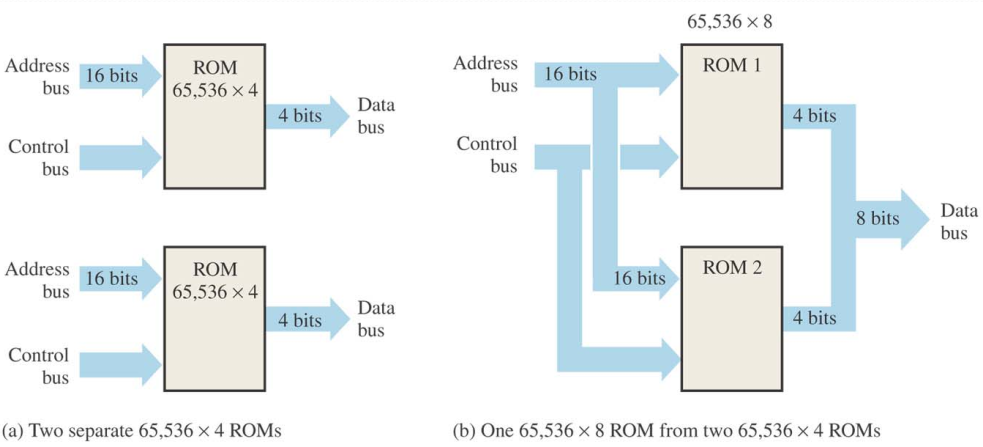
\includegraphics[width=0.6\linewidth]{fig/word-length.PNG}
\end{figure}

\subsubsection{字扩展}
\begin{itemize}
	\item 存储芯片($mk\times n$位/片)构成存储器($Mk\times n$位),需要$\lceil M/m\rceil$片
	\item 位数不变(字长不变),扩充容量(存储单元个数增加)
	\item 地址线、读写控制线对应相接,但需要加片选信号(与外部译码器相连)
\end{itemize}
\begin{figure}[H]
\centering
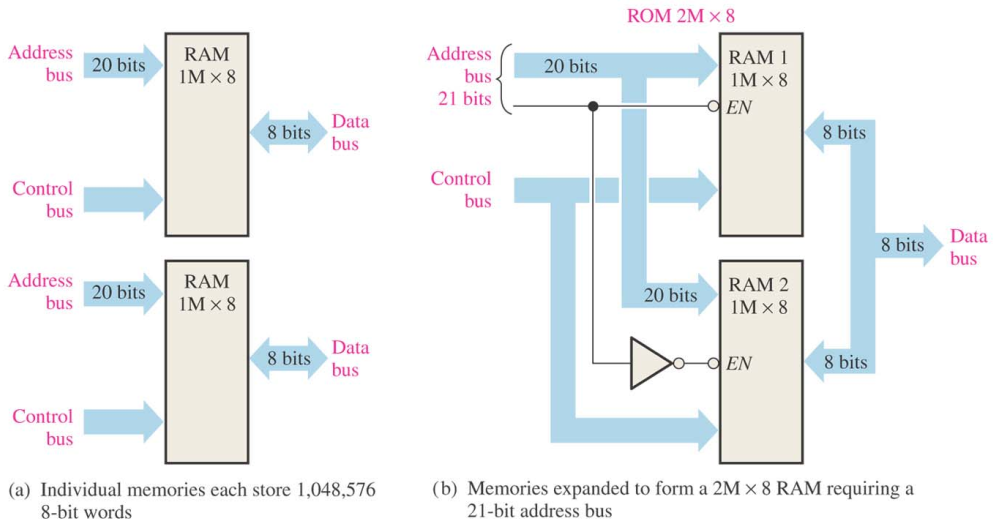
\includegraphics[width=0.6\linewidth]{fig/word-capacity.PNG}
\end{figure}

\subsubsection{字位扩展}
\begin{example}
用1K$\times$4b的DRAM芯片(64$\times$64结构)构成16K$\times$16b的存储器
\end{example}
\begin{analysis}
\begin{enumerate}
	\item 所需芯片数目:32KB/0.5KB=64
	\item 位扩展16/4=4个,字扩展16/1=16组
	\item 总共需14条地址线,因16K=$2^{14}$
	\item 其中字扩展需要4个片选信号$16=2^4$,4条线
	\item 片内寻址10条地址线
	\item 刷新周期$64T_{refresh}<T_{max}$
\end{enumerate}
\end{analysis}

\subsection{存储器与CPU的连接}
通信方式
\begin{itemize}
	\item 异步(需握手)
	\item 同步:CPU和主存由统一时钟信号控制,无需应答
\end{itemize}
主存空间的划分
\begin{itemize}
	\item ROM存放系统程序、标准子程序
	\item RAM存放用户程序
\end{itemize}
注意74LS138还有三个使能端$G_1,\overline{G_{2A}},\overline{G_{2B}}$


\subsection{Cache概述}
\subsubsection{计算机存储层次结构}
大容量、高速度、低成本\\
多级系统的存储容量即为最底层的存储容量,因为是包含关系\\
CPU与cache之间以字为单位传送,cache与主存之间以块为单位传送\\
程序访问局部性
\begin{itemize}
	\item 时间(temporal)局部性:刚被访问过的存储单元很可能不久又被访问,如循环变量
	\item 空间(spatial)局部性:刚被访问过的存储单元的邻近单元很可能不久被访问,如数组顺序访问
\end{itemize}
cache对程序员是透明的,即程序员在编写程序时无需了解cache是否存在或如何设置

\subsubsection{命中与失效}
\begin{itemize}
	\item 命中(hit):要访问的信息在cache中
	\item 失效(miss):不在cache中
\end{itemize}
平均访问时间
\[\bar{T}=pT_h+(1-p)(T_h+T_m)=T_h+(1-p)T_m\]
影响因素
\begin{itemize}
	\item cache越大,失效率越低,但成本越高
	\item block越大,失效率越低;但block在cache中所占比例增加到一定程度,失效率会上升
	\item cache容量小时,映射方式有影响;容量大时,影响不大
\end{itemize}

\subsection{cache与主存的映射}
cache存放一个主存块的对应单位为行(line)或块(block)或槽(slock)或项(entry)\\
位宽即为cache一个块的大小,如传送单位为512B,则cache每个块大小为512B\\
增大块的大小,以利用空间局部性\\
频繁的cache替换称为cache抖动

\subsubsection{直接(direct)映射}
cache内存放的内容是主存的一个子集,因此给出一个主存地址,要在cache中找到这个地址,应该将这个32位地址全部用上。末几位用于确定在cache内存储的位置,高位(tag)则用来确定是否为该地址。
\begin{itemize}
	\item 注意区别块地址、字地址、字节地址等(一般按字节编址)
	\item 按字索引则后两位不需要
	\item 先计算出块地址(因而先模块内数目),再计算块内地址
	\item $0\thicksim n-1$块称为第0区/块群,$n\thicksim 2n-1$称为第1块群,以此类推
\end{itemize}

\subsubsection{全相联(full associative)映射}
比较地址要与所有单元比较,线路复杂,成本高

\subsubsection{组相联(set associative)映射}
直接模组的数目。
相联度高,缺失率低,但会增加命中时间
只要命中了tag则对应的主存块一定在cache里
\begin{figure}[H]
\centering
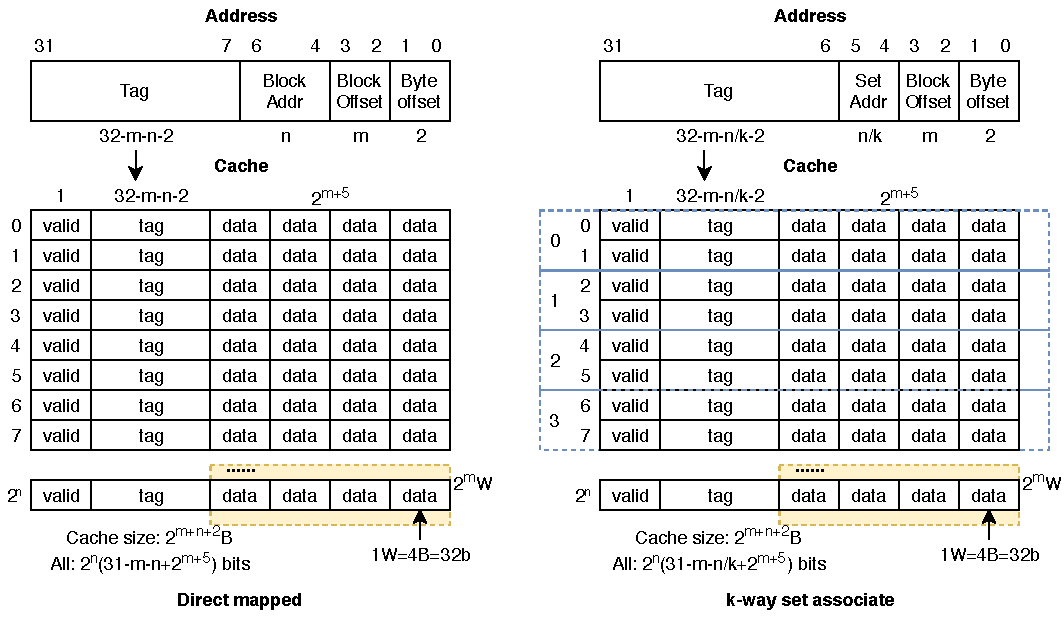
\includegraphics[width=0.8\linewidth]{fig/Cache-combine.pdf}
\end{figure}
* 不要忘记块内寻址\\
地址映射表指前面的tag和有效位部分

\begin{example}
某一直接映射的cache容量为8K字,每块内有16个字,主存容量为512K字
\end{example}
\begin{analysis}
\begin{itemize}
	\item 主存有$512K=2^{19}$个字,$512K/16=2^{19}/2^4=2^{15}$个块,$512K/8K=2^6$个区
	\item cache有$8K=2^{13}$个字,$8K/16=2^{13}/2^4=2^9$个块
	\item 主存字地址19位,区号6位,区内块号15-6=9位,块内地址4位($16=2^4$)
	\item cache字地址13位,块号9位,块内4位
	\item 主存第$i$块位于第$\lfloor i/2^9\rfloor$个区,调入cache第$i\;\mod 2^9$块
\end{itemize}
\end{analysis}


\subsection{Cache替换算法}
\begin{itemize}
	\item FIFO
	\item Least Recently Used (LRU)比较好:给每一个cache行设定一个计数器,值越小越经常被使用;不被用则加1
	\item Random
\end{itemize}

\subsection{Cache一致性}
\begin{itemize}
	\item 写命中(hit)
	\begin{itemize}
		\item 写直达(write through):同时写cache和主存\\
		加入写缓冲(write buffer),先存入写缓冲,当写主存操作结束后再将写缓冲数据释放
		\item 写回(write back):只写cache不写主存,没有同步更新!\\
		每个cache行置一个脏位(dirty bit),若cache行中的主存块被修改,则置为1;只有当脏位为1的块从cache中替换出去时才将其写回主存
	\end{itemize}
	\item 写不命中(miss)
	\begin{itemize}
		\item 写分配(allocate-on-miss):更新主存块相应单元,再将该主存块装入cache(空间局部性)
		\item 写不分配(no-allocate-on-write):直接写主存,不放回
	\end{itemize}
\end{itemize}
通常写直达+写分配/写不分配,写回+写分配

\subsection{多级Cache}
一般L1 Cache为分立Cache(数据指令分开放),减少命中时间获得较短时钟周期\\
L2 Cache为联合Cache,降低缺失率以减少主存缺失损失\\
Intel Core i7采用三级Cache
\begin{center}
\begin{tabular}{|c|c|c|}\hline
L1 & L2 & L3\\\hline
32KB I/ 32 KB D & 256KB & 2MB/core\\\hline
4-way I/8-way D & 8-way & 16-way \\\hline
Pseudo-LRU & Pseudo-LRU & \begin{tabular}{l}Pseudo-LRU\\+ordered selection algorithm\end{tabular}\\\hline
\end{tabular}
\end{center}

\subsection{虚拟存储器}
产生原因:同时运行更多进程,内存需求增大
\begin{enumerate}
	\item 允许多个程序有效而安全地共享存储器,消除内存因小而有限的容量给程序设计造成的障碍
	\begin{itemize}
		\item 可以更有效功效处理器和主存
		\item 虚存实现程序地址空间道物理空间的转换,加强了各个程序地址空间之间的保护
	\end{itemize}
	\item 允许单用户程序大小超过主存容量,虚存自动管理主存和辅存组成的两级层次结构
\end{enumerate}
\subsubsection{概述}
Cache解决系统速度,虚存解决系统容量\\
Cache全硬件管理,而虚存由硬件和OS共同管理
\begin{itemize}
	\item 将内外存统一管理的存储管理机制,按需调页(demand paging)
	\item 虚存是主存和磁盘的抽象,OS使每个进程看到的存储空间都一致
	\item 虚存为每个进程提供一个假象,好像每个进程都独占主存,且主存空间极大
\end{itemize}
\par 分页(paging)基本思想
\begin{itemize}
	\item 将内存分为固定长且较小的存储块,每个进程也划分为固定长度的程序块
	\item 程序块(页/page)可装到存储器可用的存储块(页框/page frame)中
	\item 无需用连续页框来存放一个进程,只需将当前活跃页面调入主存
	\item 操作系统为每个程序/进程生成一个页表(page table)
	\item 通过页表实现逻辑地址到物理地址的转换(address mapping)
	\item 只有进程最后一个零头(内部碎片)不能使用,浪费小
\end{itemize}
逻辑地址与物理地址区别
\begin{itemize}
	\item 逻辑地址:程序中指令所用的地址
	\item 物理地址:存放指令或数据实际内存地址
\end{itemize}
段式虚拟存储器
\begin{itemize}
	\item 段是程序本身的属性,且可以有不同长度,可自由调度
	\item 段本身是程序的逻辑结构所决定的一些独立部分,所以分段对程序员是不透明的(而分页是透明的)
	\item 但因长度可变,分配主存空间不便,容易产生内存碎片
\end{itemize}
段页式虚拟存储器
\begin{itemize}
	\item 程序按模块分段,段内再分页,进入主存仍以\textbf{页}为基本单位
	\item 逻辑地址由段地址、页地址和页内偏移量三个字段构成
	\item 用段表和页表(每段一个)进行两级定位管理
	\item 根据段地址到段表中查阅与该段相应的页表指针,再转向页表,然后根据页地址从页表中查到该页在主存中的页框地址,由此访问到页内某数据
\end{itemize}

\subsubsection{组织方式}
页式虚拟存储器,存在主存中
\begin{itemize}
	\item 指令给出虚拟地址
	\item 每个页表记录对应的虚页情况
	\item valid为0说明缺页(page fault),代价读磁盘,软件处理:当前指令执行被阻塞,当前进程挂起;缺页处理结束后,回到原指令继续执行
	\item 当读写操作不符合access right时,发生保护违例
	\item CPU执行指令时,先由内存管理单元(MMU)将逻辑地址转为物理地址
	\item 页大小比cache的block大得多,全相联映射
	\item 写回策略
\end{itemize}
页表结构
\begin{itemize}
	\item 每个进程一个页表
	\item 页表项即为页表中的一项,即物理地址(页号+页内偏移)
	\item 页表项数由进程大小决定
	\item 页表在主存的首地址记录在页表基址寄存器中
\end{itemize}
页面大小不能太小,否则页面个数多,页表太大;也不能太大,一次装入页面时间太长
\begin{example}
某页式虚拟存储器,有32位虚拟地址,页大小为4KB,每个页表项占4B,则操作系统为进程分配的页表最大为多少?
\end{example}
\begin{analysis}
最大页表项数=最多页的数目=$2^{32}/2^{12}=2^{20}$\\
最大页表大小=页表项数$\times$每个页表项大小=$2^{20}\times 2^2B$=4MB
\end{analysis}
\begin{example}
虚拟地址16位,物理地址12位,页大小为128B,TLB采用四路组相联,共16个页表项
\end{example}
\begin{analysis}
页大小$2^7$B,故7位用来做页内偏移\\
四路组相联,16个页表项,即4个组,故2位组偏移(TLB索引)\\
其余6位为TLB标志位,即$15\thicksim 7$位都为虚拟页号\\
页内偏移不变,其余用来做物理页号
\end{analysis}

\subsubsection{快表(TLB)}
转换后备缓冲器(Translation-Lookaside Buffer),存在cache中\\
每次读写操作都至少带来两次存储器访问,一次访问页表,一次访问所需的数据或指令\\
使用cache来存储页表项,它包含了最近使用的那些页表项\\
不可能页表miss了,快表hit了,因为页表缺失,信息一定不在主存页不在cache
\begin{figure}[H]
\centering
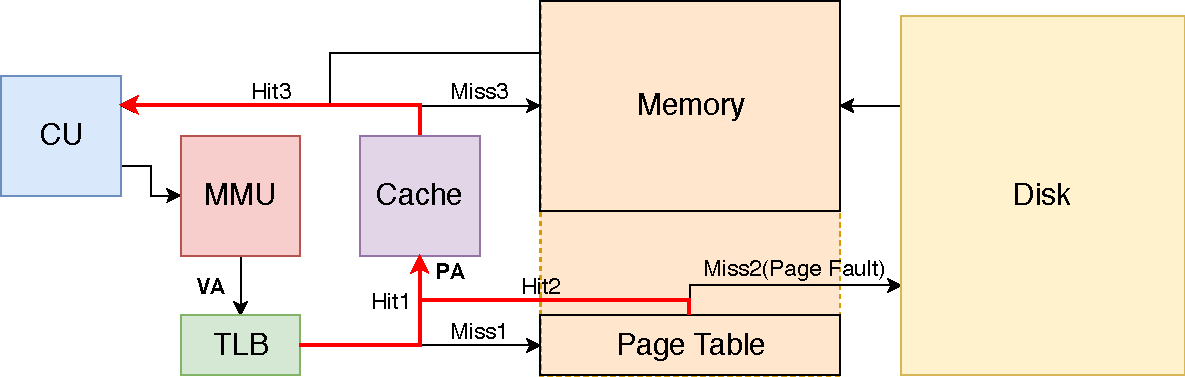
\includegraphics[width=0.6\linewidth]{fig/Cache-page.pdf}
\end{figure}
Tag即为虚拟页号=$\lceil$地址/页大小$\rceil$\\
TLB指标
\begin{itemize}
	\item 多用全相联:命中率高
	\item 采用随机替换策略:降低替换算法开销
	\item 写回策略:减少访存次数
	\item 大小:$16\thicksim 512$项
	\item 块大小:$1\thicksim 2$项(每个表项$4\thicksim 8$B)
	\item 命中时间:$0.5\thicksim 1$个时钟周期
	\item 失靶损失:$10\thicksim 100$个时钟周期
	\item 命中率:$90\thicksim 99\%$
\end{itemize}
\begin{figure}[H]
\centering
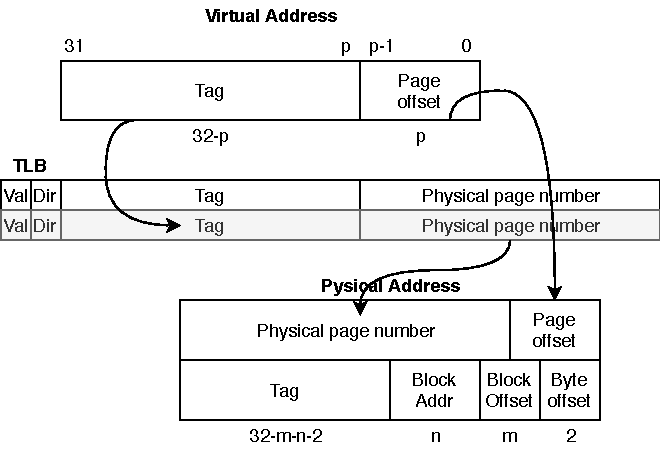
\includegraphics[width=0.5\linewidth]{fig/Cache-page_address.pdf}
\end{figure}

\subsubsection{存储保护}
\begin{itemize}
	\item 地址越界:转换到的物理地址不属于可访问范围
	\item 访问越权:访问操作所拥有的访问权限不符
\end{itemize}
通过程序重定位进行存储区域保护
\begin{itemize}
	\item 静态:在装入前将所有地址全部转为物理地址,通过给逻辑地址加界/基准地址实现
	\item 动态:由硬件地址转换机构实现
\end{itemize}

\subsection{并行主存系统}
\begin{itemize}
	\item 均匀存储访问模型(UMA, Uniform Memory Access):访问任何存储字时间相同
	\item 非均匀存储访问模型(NUMA):被共享的存储器在物理上分布于各个处理器
\end{itemize}
多处理器的cache一致性
\begin{itemize}
	\item 软件:编译使得共享数据只放在主存,不放入高速缓存
	\item 硬件:硬件协议维护,关键在于跟踪所有共享数据块的状态
	\begin{itemize}
		\item 侦听协议(snooping):侦听到主存中一个单元被修改则将自己cache中单元副本置为无效或更新
		\item 目录协议:在主存中设置一个目录表,记录共享数据的所有高速缓存行的位置和状态
	\end{itemize}
\end{itemize}